\section{Time Evolution}

    \begin{frame}[t]
        \frametitle{Goal of the Calculation}

        \begin{itemize}
            \item Evaluate the time-evolution of the system for various observables \pause
            \begin{itemize}
                \item Uses calculation in the \emph{Interaction Picture} \pause
                \item Introduce operator-less \emph{effective Hamiltonian}
            \end{itemize}
        \end{itemize}

        \vspace{1cm}

        \makebox[\textwidth][c]{
            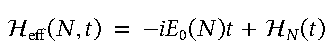
\includegraphics[width=0.165\textwidth,page=1]{main-content/time-evolution/effective-hamiltonian-definition.pdf}
            \includegraphics[width=0.45\textwidth,page=2]{main-content/time-evolution/effective-hamiltonian-definition.pdf}
        }

        % notes 
        \onslide % on all slides of frame
        \note[item] {
            TODO
        }
    \end{frame}

    \begin{frame}[t]
        \frametitle{The effective Hamiltonian}

        \makebox[\textwidth][c]{
            \includegraphics[width=0.55\textwidth,page=3]{main-content/time-evolution/effective-hamiltonian-definition.pdf}
        }

        \pause
        \begin{itemize}
            \item Constructed from the contributions of the base energy and the perturbation \pause
            \item Base energy contribution:
        \end{itemize}

        \makebox[\textwidth][c]{
            \includegraphics[width=0.65\textwidth,page=4]{main-content/time-evolution/effective-hamiltonian-definition.pdf}
        }

        % notes 
        \onslide % on all slides of frame
        \note[item] {
            TODO
        }
    \end{frame}

    \begin{frame}[t]
        \frametitle{The effective Hamiltonian}

        \begin{itemize}
            \item To evaluate the time-evolution of the perturbation
        \end{itemize}

        \makebox[\textwidth][c]{
            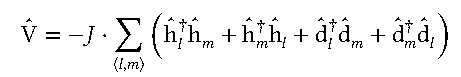
\includegraphics[width=0.50\textwidth,page=1]{main-content/time-evolution/v-in-interaction.pdf}
        }

        \pause
        \begin{itemize}
            \item Solve the equation of motion for the ladder operators
        \end{itemize}
        
        \vspace{-0.1cm}
        \makebox[\textwidth][c]{
            \includegraphics[width=0.50\textwidth,page=2]{main-content/time-evolution/v-in-interaction.pdf}
        }


        % notes 
        \onslide % on all slides of frame
        \note[item] {
            Solving the equations of motions in the interaction picture requires the number operator being \emph{idempotent}
        }
    \end{frame}

    \begin{frame}[t]
        \frametitle{The effective Hamiltonian}

        \begin{itemize}
            \item Insert and reorder the operators
        \end{itemize}

        \makebox[\textwidth][c]{
            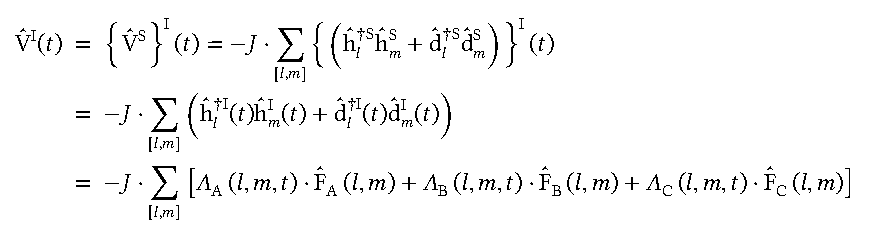
\includegraphics[width=0.80\textwidth,page=1]{main-content/time-evolution/v-in-interaction-solution.pdf} % TODO
        }%
        \vspace{-0.0cm}
        \pause
        \makebox[\textwidth][c]{
            \includegraphics[width=0.80\textwidth,page=2]{main-content/time-evolution/v-in-interaction-solution.pdf}
        }

        % notes 
        \onslide % on all slides of frame
        \note[item] {
            TODO
        }
    \end{frame}

    \begin{frame}[t]
        \frametitle{The effective Hamiltonian}

        \begin{itemize}
            \item Evaluate the contribution to the effective Hamiltonian \pause
            \begin{itemize}
                \item Requires previously calculated value of the V-operator in the Interaction Picture \pause
                \item Controllable \emph{cumulant expansion}
            \end{itemize}
        \end{itemize}

        \pause[2]
        \vspace{0.2cm}
        \makebox[\textwidth][c]{
            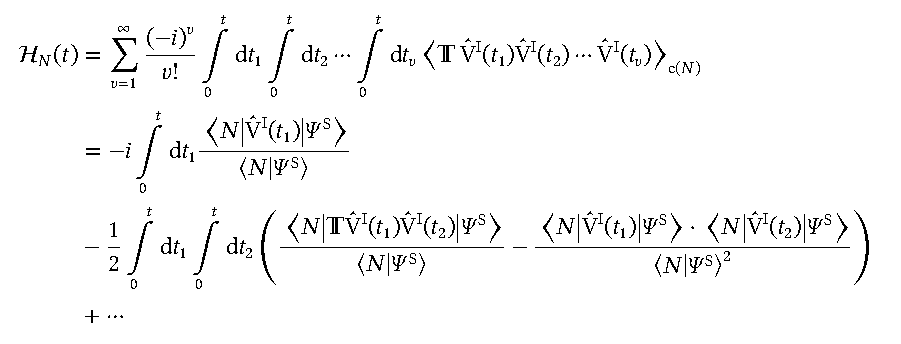
\includegraphics[width=0.80\textwidth,page=1]{main-content/time-evolution/effective-hamiltonian-n.pdf}
        }

        % notes 
        \onslide % on all slides of frame
        \note[item] {
            TODO
        }
    \end{frame}

    \begin{frame}[t]
        \frametitle{Handling of Observables}

        \begin{itemize}
            \item This allows for general evaluation of expectation values \pause
            \begin{itemize}
                \item Requires a transition probability
                \item Requires a local observable
            \end{itemize}
        \end{itemize}

        \pause[1]
        \vspace{0.2cm}
        \makebox[\textwidth][c]{
            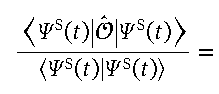
\includegraphics[width=0.28\textwidth,page=1]{main-content/time-evolution/time-evolution-of-observable.pdf}
        }
        \pause[2]
        \makebox[\textwidth][c]{
            \includegraphics[width=0.80\textwidth,page=2]{main-content/time-evolution/time-evolution-of-observable.pdf}
        }

        % notes 
        \onslide % on all slides of frame
        \note[item] {
            Does only require difference of effective Hamiltonian for evaluation (notice for later)
        }
    \end{frame}

    \begin{frame}[t]
        \frametitle{Simple Observalbles}

        \begin{itemize}
            \item Local observable for double occupation measurement \pause
            \begin{itemize}
                \item Observables generally are very sparse matrices
                \item Reduces to pure occupation measurement
            \end{itemize}
        \end{itemize}

        \makebox[\textwidth][c]{
            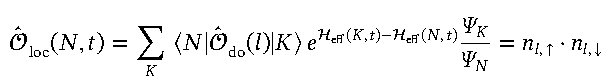
\includegraphics[width=0.7\textwidth,page=1]{main-content/time-evolution/local-observables-simple-ops.pdf}
        }

        \pause
        \begin{itemize}
            \item Local observable for particle current measurement \pause
            \begin{itemize}
                \item Requires evaluation of the difference of two effective Hamiltonians
            \end{itemize}
        \end{itemize}

        \makebox[\textwidth][c]{            
            \includegraphics[width=0.8\textwidth,page=2]{main-content/time-evolution/local-observables-simple-ops.pdf}
        }

        % notes 
        \onslide % on all slides of frame
        \note[item] {
            Complex observable, make sure this cancels
        }
    \end{frame}

    \begin{frame}[t]
        \frametitle{Access to Density-Matrics}

        \begin{itemize}
            \item Non-classical (\emph{quantum}) measurements depend on the (reduced) density matrix \pause
                \begin{itemize}
                    \item Access to \emph{purity}, \emph{concurrence} and other entanglement measures/monotones\pause
                \end{itemize}
            \item Direct calculation not possible
        \end{itemize}

        \vspace{-0.2cm}
        \makebox[\textwidth][c]{
            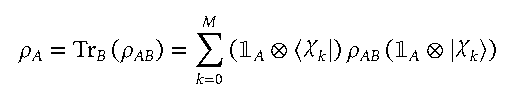
\includegraphics[width=0.65\textwidth,page=1]{main-content/time-evolution/reduced-density-matrix.pdf}
        }

        \vspace{-0.2cm}
        \pause
        \begin{itemize}
            \item Use Pauli matrices to expand the complex 4x4 matrix
        \end{itemize}

        \makebox[\textwidth][c]{
            \includegraphics[width=0.65\textwidth,page=2]{main-content/time-evolution/reduced-density-matrix.pdf}
        }

        % notes 
        \onslide % on all slides of frame
        \note[item] {
            TODO
        }
    \end{frame}

    \begin{frame}[t]
        \frametitle{Access to Density-Matrics}

        \makebox[\textwidth][c]{
            \includegraphics[width=0.75\textwidth,page=3]{main-content/time-evolution/reduced-density-matrix.pdf}
        }

        % notes 
        \onslide % on all slides of frame
        \note[item] {
            TODO
        }
    \end{frame}